\documentclass[10pt,a4paper]{article}
\usepackage{fontspec,amsmath,amssymb,amsthm,mathtools,graphicx,bm,bbm,stmaryrd,nicefrac,braket,xcolor}
\usepackage[margin=22mm]{geometry}
\usepackage[bookmarks=false]{hyperref}
\setlength{\emergencystretch}{3em}\newcommand{\absolutevalue}[1]{\left|#1\right|}\newcommand{\norm}[1]{\left\lVert#1\right\rVert}
\title{Sharper weighted adversary bound for non-adaptive non-collapsing quantum queries}
\author{David Miloschewsky, Supartha Podder}
\date{doi:10.4230/LIPIcs.CCC.2025.12; CC BY 4.0}
\begin{document}
\maketitle
\noindent\textit{Editorial note.} Editable TeX converted from the official CC BY HTML prose and math alttext. Original official PDF/HTML retained. Only the specified claim counts; all author context and available source-local supporting proofs are included.\par\medskip
\noindent\textit{Editorial note.} Author notation retained: cached official HTML TeX alttext S5.Ex52.m1 (Lemma24 statement) has wt(x)/v(y,i) and wt(y)/v(x,i), while S5.E28.m1 (first displayed inequality in its proof) has wt(x)/v(x,i) and wt(y)/v(y,i). The converted source at lines1477 and1496 retains these respective original expressions. This records the source notation only; no author formula is changed.\par\medskip


\par\medskip\noindent\textbf{
1 Introduction}\par




\par\medskip\noindent\textbf{
1.1 Background and motivation}\par




The study of the quantum query complexity model has lead to a rewarding avenue of research in understanding quantum speed-ups [29, 12, 11, 19]. In this model, one is given access to an input $x$ through a black-box and the goal is to evaluate $f(x)$ for some function $f$ while minimizing the number of quantum queries to $x$. A variety of tools have been developed to lower-bound quantum query complexity, notably the polynomial method [11], where one uses the fact that a polynomial may describe the amplitudes of a quantum state, the hybrid method [12] and its generalization the adversary method [7, 33], which quantifies the difficulty of distinguishing between inputs with different images. The study and application of these techniques has been instrumental in understanding the complexity class characterizing quantum computation, $\mathsf{BQP}$ (Bounded-error Quantum Polynomial-time). Specifically, as one may be given access to $x$ through an oracle $O$, quantum query complexity studies $\mathsf{BQP}^{O}$ and its relations to other complexity classes with access to $O$.\par




One of the goals of studying $\mathsf{BQP}$ is to characterize the classes of functions which may be efficiently computable once fault-tolerant quantum computers have been realized. The difficulty of this realization and the need to mimic our current hardware has lead us to place various restrictions on $\mathsf{BQP}$. One prominent issue, the presence of noise, motivated the study of noise in the quantum query complexity setting, i.e., to introduce noise to the oracle calls. This was explored in [26], where the authors showed that Grover’s algorithm loses its speed-up even if only a single qubit is randomly affected with depolarizing noise. Furthermore, [14] defined the class $\mathsf{NISQ}$ (Noisy Intermediate-Scale Quantum), the class of problems solved by a $\mathsf{BPP}$ algorithm with access to a noisy quantum device, emulating some aspects of today’s state of quantum computation. They showed an oracle separation between both $\mathsf{BPP}$ and $\mathsf{BQP}$, and showed that $\mathsf{NISQ}$ algorithms cannot solve search as fast as $\mathsf{BQP}$.
These results point to the conclusion that the presence of noise considerably weakens the computational power.\par




Another intriguing limited setting of the query model is the non-adaptive query model [23]. Here we restrict the model to a single round a parallel queries and analyze the necessary width of the round, imposing that the queries are independent of each other. It was shown in [23] that this restriction thwarts the quantum speed-up in solving the search and element distinctness problems, implying that adaptivity is necessary in order to obtain polynomial speed-ups for some problems.\par




On the other hand, augmenting $\mathsf{BQP}$ with a metaphysical ability have also been a fruitful avenue in understanding the power of computation.
One of the first considered variations of quantum mechanics was adding post-selection to quantum computation, $\mathsf{PostBQP}$ (Post-selected $\mathsf{BQP}$). Post-selection is the ability that, given a quantum state, we may \emph{select} a partial measurement outcome, regardless of its probability. It was shown that $\mathsf{PostBQP}=\mathsf{PP}$ [2], establishing an equivalency between a quantum and classical computational class. However, $\mathsf{PostBQP}$ is well above $\mathsf{BQP}$ as even $\mathsf{QMA}$, a quantum version of $\mathsf{NP}$, is contained in $\mathsf{PP}$.\par




One of the theories explaining quantum mechanics is the hidden variable theory, an interpretation where the system is described by a state and a hidden variable which stochastically determines the measurement results. $\mathsf{DQP}$ (Dynamical Quantum Polynomial-time) is defined as the set of languages solved by a classical deterministic polynomial-time Turing machine which can process the history of the hidden variables of a quantum algorithm [1]. At the moment, we only know that $\mathsf{BQP}\subseteq\mathsf{DQP}\subseteq\mathsf{EXP}$ and the best known search algorithm uses $O(N^{1/3})$ queries. However, [5] showed that adjusting $\mathsf{DQP}$ to $\mathsf{CDQP}$ (Circuit-indifferent $\mathsf{DQP}$), adding a restriction to the hidden variable theory, gives us a $\Omega(N^{1/4})$ lower-bound on search.\par




A well-studied offspring of $\mathsf{DQP}$ is $\mathsf{PDQP}$ (Product Dynamical Quantum Polynomial-time), quantum computation powered with non-collapsing measurements. By non-collapsing measurements, we mean that given an arbitrary state $\ket{\psi}$, we sample a measurement result without collapsing the state.
We may view this as a simplification of $\mathsf{DQP}$ as we are given samples from the history of computation. Defined in [5], the authors proved a $\Omega(N^{1/4})$ lower-bound on search and $\mathsf{SZK}\subseteq\mathsf{PDQP}\subseteq\mathsf{BPP}^{\mathsf{PP}}$.\par




A class related to $\mathsf{PDQP}$ is $\mathsf{CBQP}$ (Copy $\mathsf{BQP}$), $\mathsf{BQP}$ with the ability to create an unentangled copy of any state. Note that $\mathsf{CBQP}$ can simulate non-collapsing measurement by creating a copy and measuring it. However, the ability to entangle copies together adds considerable power. It was shown that $\mathsf{CBQP}$ can solve any $\mathsf{NP}$-hard problem in polynomial time using a single query and $O(\log(N))$ copies [9]. The class is positioned between $\mathsf{BQP}^{\mathsf{PP}}$ and $\mathsf{PSPACE}$ [21].\par




In our work, we revisit $\mathsf{PDQP}$ as, except for $\mathsf{CDQP}$, it is known to be only slightly stronger than $\mathsf{BQP}$ as it may at most attain a polynomial speed-up over Grover’s algorithm. To understand the lower-bound, we must first describe a caveat. In the standard quantum query model, the goal is to minimize the amount of queries $Q$. However, in models with an additional ability, such as creating a copy or performing a non-collapsing measurement, we must provide bounds on the uses of the ability, which we denote by $P$. In the case of non-collapsing measurements, without minimizing both $Q$ and $P$, every problem of size $N$ could be trivially solved using a single query and followed by exponentially-many non-collapsing measurements which are repeated until we learn enough information about the input. Furthermore, unrestricted non-collapsing measurements lead to quantum cloning, faster than light communication and constant communication complexity [5]. Therefore the measure of complexity is $Q+P$, the sum of the number of queries and number of non-collapsing measurements.\par




The search lower-bound may lead some to the conclusion that a $\mathsf{PDQP}$ algorithm with $P$ non-collapsing measurements may be simulated by $\mathsf{BQP}$ with a squared overhead by running $P$ separate computations in parallel. However, this intuition fails as the \emph{deferred measurement principle} does not hold in $\mathsf{PDQP}$. To explain why, consider the collision problem. Here, assuming $N\in\mathbb{N}$, one is given black-box access to a function $f:[N]\rightarrow[N]$ with the promise that for any $x\in[N]$, $k=|\{y:f(y)=f(x)\}|$ is either 1 or 2. The algorithm is as follows. First, we query all the indices into a superposition and call the oracle, obtaining,\par


\[\begin{gathered}
\displaystyle\ket{\psi^{\prime}}=\sum_{x\in[N]}\ket{x}\ket{f(x)}
\end{gathered}\]


Next, we measure the query output register, collapsing $\ket{\psi^{\prime}}$ to $\ket{\psi}$ and obtaining $f(x_{1})$ as our measurement result. We find ourselves with the following state,\par


\[\begin{gathered}
\displaystyle\ket{\psi}=\begin{cases}\ket{x_{1}}\ket{f(x_{1})}&\text{if }k=1\\
\frac{\ket{x_{1}}+\ket{x_{2}}}{\sqrt{2}}\ket{f(x_{1})}&\text{if }k=2\end{cases}
\end{gathered}\]




By repeating $O(1)$ non-collapsing measurements of $\ket{\psi}$, we find $k$ with high probability, solving the problem with both constant queries and non-collapsing measurements. On the other hand, without the partial measurement, the algorithm is no longer efficient. In contrast, $\tilde{\Theta}(N^{1/3})$ queries are optimal in $\mathsf{BQP}$ [13, 28]. Note that the proof of $\mathsf{SZK}\subseteq\mathsf{PDQP}$ uses the same partial measurement trick to solve the Statistical Difference problem, which is $\mathsf{SZK}\text{-hard}$ [27].\par




When it was introduced, $\mathsf{PDQP}$ was referred to as $\mathsf{naCQP}$ (non-adaptive Collapse-free Quantum Polynomial-time). The class $\mathsf{naCQP}$ is a restriction of $\mathsf{CQP}$, the class with the ability to adapt the quantum computation based on the non-collapsing measurement results. The power of this class is unknown as there are no known algorithms which utilize the adaptive feature nor do we have any lower-bounds. We note that that the phrase \emph{non-adaptive} in $\mathsf{naCQP}$ is not related to non-adaptive queries discussed above, $\mathsf{naCQP}$ has the ability to perform a query at any step of the algorithm.\par




Recently, non-collapsing measurements gained renewed interest. It was shown that the complexity class $\mathsf{PDQMA}$ (Product Dynamical Quantum Merlin-Arthur), the quantum counter-part of $\mathsf{NP}$ with the power of non-collapsing measurements, equals $\mathsf{NEXP}$ [6, 10]. Inspired by their work and several open directions in the original $\mathsf{PDQP}$ literature, we revisit the class.
There are several settings to study $\mathsf{PDQP}$ in. One may focus on adapting unitaries based on non-collapsing measurement results, restricting the query adaptivity or limiting partial measurements. We explore the power of non-collapsing measurements with non-adaptive queries. To avoid any confusion, for the remainder of the paper, any discussion of non-adaptability will be concerned with queries.\par




It is important to stress that the point of these adjustments is not to argue for alterations of the postulates of quantum mechanics. Instead, we explore quantum computation and complexity from an alternative point. Therefore, the models we define to encompass the adjustments of $\mathsf{BQP}$ may use ideas which are not inherently present in quantum computation. This is unavoidable as if they could be described solely using the postulates of quantum mechanics, their complexity class would be equal to $\mathsf{BQP}$.\par





\par\medskip\noindent\textbf{
1.2 Results}\par




\par\medskip\noindent\textbf{
1.2.1 Lower-bounding methods}\par




We obtain a trade-off between queries and non-collapsing measurements by developing the adversary method lower-bound in our setting. For simplicity, our results are presented using the basic adversary method from [7], but we prove its generalization, the positive weighted adversary method of [8] (see Subsection 7.1). When discussing query complexity, we will use the name of the complexity class as the identifier of the model. We note that in all cases, one recovers the original adversary method by setting the number of non-collapsing measurements to 1, essentially only measuring the end state. The result below exhibits that non-collapsing measurements provide us with a limited speed-up over $\mathsf{BQP}$ in problems which may be lower-bounded by the positive weighted adversary method.\par



% SOURCE-ID Thmtheorem1


\par\medskip\noindent\textbf{
\textbf{Result 1}\textbf{ }(\textbf{Adversary method on BQP with non-collapsing measurements}, directly from Lemma 18)\textbf{.}
}\par



\emph{Let $f:\{0,1\}^{|\Sigma|}\rightarrow\{0,1\}$ be a boolean function and $x$ an input.
Define $X\subseteq f^{-1}(0)$, $Y\subseteq f^{-1}(1),R\subseteq X\times Y$. Based on $X,Y,R$, let $m,m^{\prime}$ be the minimum number of elements $(x,y)$ for each $x\in X$ and $y\in Y$ respectively and $l,l^{\prime}$ are the most elements $(x,y)$ where $x(i)\neq y(i)$ for each $i\in\Sigma$ and for each $x\in X$ and $y\in Y$ respectively.}\par




\emph{Any algorithm solving $f(x)$ in a $\mathsf{PDQP}$ setting with $Q$ queries and $P$ non-collapsing measurements satisfies,}\par


\[\begin{gathered}
\displaystyle QP=\Omega\left(\sqrt{\frac{mm^{\prime}}{ll^{\prime}}}\right)
\end{gathered}\]



% END-SOURCE-ID Thmtheorem1



We develop a similar trade-off between $Q$ and $P$ in the non-adaptive query setting. Defined in Subsection 5.1, we denote it with the superscript $nq$.\par



% SOURCE-ID Thmtheorem2


\par\medskip\noindent\textbf{
\textbf{Result 2}\textbf{ }(\textbf{Adversary method on non-adaptive BQP with non-collapsing measurements}, directly from Lemma 24)\textbf{.}
}\par



\emph{Define $f,x,m,m^{\prime},l,l^{\prime}$ as in Result 1. Any algorithm solving $f(x)$ in a $\mathsf{PDQP}^{nq}$ setting with $Q$ queries and $P$ non-collapsing measurements satisfies,}\par


\[\begin{gathered}
\displaystyle QP=\Omega\left(\max\left\{\frac{m}{l},\frac{m^{\prime}}{l^{\prime}}\right\}\right)
\end{gathered}\]



% END-SOURCE-ID Thmtheorem2



Additionally, we obtained a variation of Result 1 for $\mathsf{CBQP}$ by applying a similar proof technique.\par



% SOURCE-ID Thmtheorem3


\par\medskip\noindent\textbf{
\textbf{Result 3}\textbf{ }(\textbf{Adversary method on BQP with the ability to copy states}, directly from Lemma 26)\textbf{.}
}\par



\emph{Define $f,x,m,m^{\prime},l,l^{\prime}$ as in Result 1. Any algorithm solving $f(x)$ in a $\mathsf{CBQP}$ setting with $Q$ queries and $P$ copies satisfies,}\par


\[\begin{gathered}
\displaystyle Q\cdot 2^{P}=\Omega\left(\sqrt{\frac{mm^{\prime}}{ll^{\prime}}}\right)
\end{gathered}\]



% END-SOURCE-ID Thmtheorem3




\par\medskip\noindent\textbf{
1.2.2 Applications of the lower-bounding methods}\par



Table 1: Summary of bounds on all the computational models explored. The non-trivial bounds we establish or improve in this paper are colored red. The $\mathsf{BQP}$ bounds are added for reference.




 
$\mathsf{BQP}$ 
$\mathsf{PDQP}$ 
$\mathsf{PDQP}^{nq}$ 
\par



 \textbf{Unstructured search}
 
$\tilde{\Theta}(\sqrt{N})$ 
$\color[rgb]{0.546875,0,0}\definecolor[named]{pgfstrokecolor}{rgb}{0.546875,0,0}\tilde{\Theta}(N^{1/3})$ 
$\color[rgb]{0.546875,0,0}\definecolor[named]{pgfstrokecolor}{rgb}{0.546875,0,0}\tilde{\Theta}(\sqrt{N})$ 
\par


\textbf{Majority} 
$\Theta(N)$ 
$\color[rgb]{0.546875,0,0}\definecolor[named]{pgfstrokecolor}{rgb}{0.546875,0,0}\tilde{\Theta}(\sqrt{N})$ 
$\color[rgb]{0.546875,0,0}\definecolor[named]{pgfstrokecolor}{rgb}{0.546875,0,0}\tilde{\Theta}(\sqrt{N})$ 
\par



\textbf{Collision}
 
$\tilde{\Theta}(N^{1/3})$ 
$\Theta(1)$ 
$\Theta(1)$ 
\par


\textbf{Element distinctness} 
$\tilde{\Theta}(N^{2/3})$ 
$\color[rgb]{0.546875,0,0}\definecolor[named]{pgfstrokecolor}{rgb}{0.546875,0,0}O(\sqrt{N})$ 
$\color[rgb]{0.546875,0,0}\definecolor[named]{pgfstrokecolor}{rgb}{0.546875,0,0}\tilde{\Theta}(\sqrt{N})$ 
\par


$\color[rgb]{0.546875,0,0}\definecolor[named]{pgfstrokecolor}{rgb}{0.546875,0,0}\Omega(N^{1/4})$ 
\par







We apply the results above to specific problems in order to draw inference about $\mathsf{PDQP}$. Specifically, we consider the bounds on search, majority and element distinctness in the settings discussed above. A summary of the bounds is in Table 1. Proof of the applications of the bounds above may be found in Subsection 7.1.\par




In the search problem, we are given access to a function $f:[N]\rightarrow\{0,1\}$ and the goal is to decide whether there exists an $x\in[N]$ such that $f(x)=1$. The lower-bound on search in $\mathsf{PDQP}$ was one of the main results in [5], but it was not tight. As the method in Result 1 provides us with the same lower-bound, we prove a tighter bound in Lemma 19.\par



% SOURCE-ID Thmtheorem4


\par\medskip\noindent\textbf{
\textbf{Result 4}\textbf{ }(\textbf{Bounds on search})\textbf{.}
}\par



\emph{We obtain tight bounds for unstructured search. In $\mathsf{PDQP}$, the bound is $\tilde{\Theta}(N^{1/3})$, while in $\mathsf{PDQP}^{nq}$ it is $\tilde{\Theta}(\sqrt{N})$.}\par



% END-SOURCE-ID Thmtheorem4



Next, we consider the majority problem. In this problem, assuming $n\in\mathbb{N}$ and $N=2^{n}$, we are given $f:[N]\rightarrow\{0,1\}$ and must decide whether $s=|\{x:f(x)=1\}|\geq 2^{n-1}$. As majority may be solved efficiently in $\mathsf{PP}$, we obtain an oracle separation between $\mathsf{PP}$ and $\mathsf{PDQP}$.\footnote{The lower-bound on search implies a separation between $\mathsf{NP}$ and $\mathsf{PDQP}$, therefore implying this separation. However, we don’t expect majority to separate $\mathsf{PDQP}$ and $\mathsf{NP}$ nor $\mathsf{QMA}$.}\par



% SOURCE-ID Thmtheorem5


\par\medskip\noindent\textbf{
\textbf{Result 5}\textbf{ }(\textbf{Bounds on majority})\textbf{.}
}\par



\emph{We obtain tight bounds for the majority problem. In both $\mathsf{PDQP}$ and $\mathsf{PDQP}^{nq}$, it is $\tilde{\Theta}(\sqrt{N})$.}\par



% END-SOURCE-ID Thmtheorem5



While the collision problem has $O(1)$ bounds, it is interesting that the same is not the case for the element distinctness problem. The problem is to decide, given $f:[N]\rightarrow[N]$, whether there exist $x,y$ such that $x\neq y$ and $f(x)=f(y)$. In $\mathsf{BQP}$, we have a clear connection between the two classes, as their bounds may be derived from each other [15]. However, this is not the case in any $\mathsf{PDQP}$ setting. It would be very interesting to characterize what causes this difference.\par



% SOURCE-ID Thmtheorem6


\par\medskip\noindent\textbf{
\textbf{Result 6}\textbf{ }(\textbf{Bounds on element distinctness})\textbf{.}
}\par



\emph{We obtain bounds for the element distinctness problem. In $\mathsf{PDQP}$, the bound is between $O(\sqrt{N})$ and $\Omega(N^{1/4})$, while in $\mathsf{PDQP}^{nq}$ it is $\tilde{\Theta}(\sqrt{N})$.}\par



% END-SOURCE-ID Thmtheorem6



Finally, let us consider the $\mathsf{CBQP}$ setting.  [9] showed an algorithm which uses a single query and $O(\log(N))$ copies to solve the search problem. Applying Result 3 shows that this algorithm is optimal.\par






\par\medskip\noindent\textbf{
1.3 Proof techniques}\par




We describe the ideas behind our proofs. The key part of this paper is Definition 13, an alternative definition of the $\mathsf{PDQP}$ model. It allowed us to prove Lemma 15, enabling us to ignore partial measurement in the proofs of our lower-bounds.\par



\par\noindent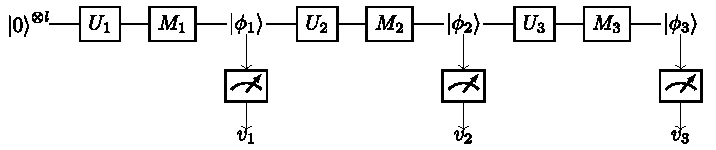
\includegraphics[width=\linewidth,height=0.78\textheight,keepaspectratio]{ccc2025-12-svg-01.pdf}\par

Figure 1: Example of the process of the oracle $\mathcal{Q}_{P}$ with $P=3$. Given a circuit $C$, the oracle $\mathcal{Q}_{P}$ returns $\{v_{i}\}_{i}^{3}$ by measuring the states $\{\phi_{i}\}_{i}^{3}$ at each step of $C$.



\par\medskip\noindent\textbf{
1.3.1 Alternative definition of computation with non-collapsing measurements}\par




Before explaining our alternative definition, we discuss the original definition of the model with non-collapsing measurements from [5]. $\mathsf{PDQP}$ is defined as the set of languages solvable by a deterministic Turing machine with one query to an oracle $\mathcal{Q}_{P}$, which runs a quantum circuit $C$ with $P$ steps. At step $i$, when the computation is in the state $\ket{\phi_{i}}$, the oracle obtains a measurement sample $v_{i}$ of $\ket{\phi_{i}}$ without collapsing it. At the end, the machine receives $\{v_{i}\}_{i}$ and processes it. An example of how the oracle runs $C$ is in Figure 1. We define an alternative oracle $\mathcal{Q}_{P}^{*}$ which inputs circuit $C$ and outputs $\{v_{i}\}_{i}$ as well. However, we explicitly describe the quantum circuit $C^{*}$ which $\mathcal{Q}_{P}^{*}$ runs. The goal is to describe $C^{*}$ such that it outputs the tensor product of each state before the non-collapsing measurement. Therefore, we may obtain the results by measuring the end state.\par




Assume the input circuit $C$ is an alternating combination of unitaries $U_{i}$ and (potentially empty) partial measurement gates $M_{i}$. We create the variants $U^{*}_{i}$ and $M^{*}_{i}$ of these gates in $C^{*}$. The goal is that at every step $i$, we have $r_{i}=P-i+1$ copies of the state $\ket{\phi_{i}}$ and our gates affect $r_{i}$ states, each of whose goal is to end in $\ket{\phi_{j}}$ where $j\geq i$. An example of the circuit $C^{*}$ is in Figure 2. The unitary $U^{*}_{i}$ is a parallel application of $U_{i}$ over each of the $r_{i}$ registers separately. The measurement $M^{*}_{i}$ is more complex as it must ensure that the partial measurement results are the same for all $r_{i}$ registers in order for them to remain copies of each other. We define it as a gate which may post-select on measuring the same outcome for each register with an adjusted probability distribution.\par




Let us explain the probability adjustment. Suppose we are measuring a single qubit in each register and want to ensure that we measure $\ket{0}^{\otimes r_{i}}$ or $\ket{1}^{\otimes r_{i}}$. Let the probability of measuring 1 at step $i$ of $C$ be $a$. If we post-selected on this to happen in a $\mathsf{PostBQP}$ manner, the probability of measuring $1^{\otimes r_{i}}$ is $\frac{a^{r_{i}}}{a^{r_{i}}+(1-a)^{r_{i}}}$, not $a$ as desired. Therefore we must adjust the probabilities of measuring $1^{\otimes r_{i}}$ by $d=a^{r_{i}-1}$.\footnote{This is the reason why it is difficult to directly show $\mathsf{PDQP}\subseteq\mathsf{PostBQP}$.} It is important to mention that $M^{*}_{i}$ is not a valid quantum operator as its projectors don’t sum to the identity. The only measurement which is allowed by quantum mechanics is the measurement of the states at the end of $C^{*}$. This is why $\mathsf{PDQP}$ is more powerful than $\mathsf{BQP}$.\par





\par\medskip\noindent\textbf{
1.3.2 Obtaining the lower-bounding techniques}\par




Using our alternative definition, we show in Lemma 15 that given two arbitrary states $(\rho_{1,i},\rho_{2,i})$ created by $C^{*}$, applying $M^{*}_{i}$ cannot decrease the fidelity between them. Our adversary method uses fidelity as the progress measure, implying that we may ignore the effect of partial measurement during our proof. Finally, we obtain a positive weighted adversary method [8] for our model by closely following the original proof while accounting for the presence of copies of states, obtaining Lemma 18.\par




Our remaining lower-bounds use the lemmata we proved above. First, our result on non-adaptive queries with non-collapsing measurements is described in Lemma 22. The proof combines the original adversary method proof for non-adaptive queries [23], replacing the original positive weighted adversary with Lemma 18. Second, our tight $\Omega(N^{1/3})$ lower-bound on search in Lemma 19 is a direct extension of the proof on search in $\mathsf{PDQP}$ with no partial \emph{collapsing} measurements (Appendix E in [5]) combined with our ability to ignore the effect of partial measurements which comes directly from Lemma 15.\par




Additionally, we apply the same idea of using non-standard gates to describe a computational model in order to obtain a lower-bounding technique for quantum computation with copies, $\mathsf{CBQP}$. The techniques remain the same as above, except we allow for the entanglement between copies instead of instantly collapsing them.\par



\par\noindent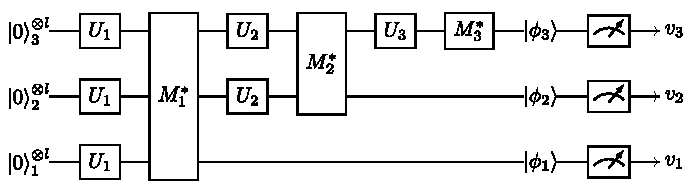
\includegraphics[width=\linewidth,height=0.78\textheight,keepaspectratio]{ccc2025-12-svg-02.pdf}\par

Figure 2: Example of the circuit $C^{*}$ with $P=3$ which is run by oracle $\mathcal{Q}_{P}^{*}$, producing the same results as oracle $\mathcal{Q}_{P}$.





\par\medskip\noindent\textbf{
1.4 Related work}\par




Since the introduction of non-collapsing measurements [5], there have been several papers analyzing the adjustment in other settings. Specifically, we have $\mathsf{PDQP/qpoly}=\mathsf{ALL}$ [4] and $\mathsf{PDQMA}=\mathsf{NEXP}$ [6, 10]. Furthermore, it was shown in [20] that there exists an oracle $O$ such that $\mathsf{P}^{O}=\mathsf{BQP}^{O}=\mathsf{SZK}^{O}=\mathsf{PDQP}^{O}\neq(\mathsf{UP}\cap\mathsf{coUP})^{O}$ and that relative to a random oracle $O$, $\mathsf{NP}^{O}\not\subseteq\mathsf{PDQP}^{O}$. Finally, [16] studied the effect on quantum theory when we may \emph{only} perform non-collapsing measurements, meaning we may never collapse a quantum state.\par




Another alteration worth mentioning is adding the power to rewind from a collapsed result back to the state prior to measurement. Denoted $\mathsf{RwBQP}$ (Rewindable $\mathsf{BQP}$), it was shown to be equal to $\mathsf{CBQP}$ and $\mathsf{AdPostBQP}$ (Adaptive $\mathsf{PostBQP}$) [21]. Adaptivity in $\mathsf{AdPostBQP}$ means that based on partial measurement outcomes, we adapt the post-selection. Equivalently, $\mathsf{RwBQP}$ may be described as $\mathsf{PDQP}$ with the additional power to decide whether, once we obtain a non-collapsing measurement, we collapse the state to that sample. This means that adding some form of adaptivity to $\mathsf{PostBQP}$ and $\mathsf{PDQP}$ makes them equivalent.\par




Furthermore, $\mathsf{PDQP}$ without partial measurements may be viewed as $\mathsf{BQP}$ with parallel queries. Various bounds on this setting have been developed, such as for Grover’s algorithm [32] and the general adversary method [22].\par




Closely related to parallel queries is adaptivity as non-adaptive algorithms have a single parallel query. Adaptivity of $\mathsf{BQP}$ queries has been a subject of prior research. The positive weighted adversary method was adjusted for non-adaptive queries [23] and it was shown that total functions depending on $N$ variables require $\Omega(N)$ queries to the input [24]. Both results showed that non-adaptivity restricts the speed-ups quantum algorithms may achieve. Related to this, the analysis of the number of adaptive queries was studied in [18], where the authors showed that for any $r\in\mathbb{N}$, the $2r$-fold Forrelation problem can be solved with $r$ adaptive rounds using one query per round, while $r-1$ adaptive round would require an exponential number of queries per round.\par





\par\medskip\noindent\textbf{
1.5 Open problems}\par




We list several open questions worth pursuing below.\par


\begin{itemize}


\item[] 
$\blacksquare$ 


In $\mathsf{BQP}$, the bounds between the collision problem and the element distinctness problem are polynomially related. Our results show that this is not true in $\mathsf{PDQP}$. Is it possible to characterize the reason behind this stark difference? We note that it is something which is not recognizable by any $\mathsf{BQP}$ algorithm.\par





\item[] 
$\blacksquare$ 


All efforts to lower-bound the query complexity of $\mathsf{PDQP}$ used methods derived from $\mathsf{BQP}$. Is it possible to develop lower-bounding techniques which are tailored for non-collapsing measurements? Similarly, is it possible to obtain lower-bounds using an altered version of the polynomial method\footnote{We discuss this in Subsection 7.2}?\par





\item[] 
$\blacksquare$ 


How does $\mathsf{PDQP}$ or other metaphysical classes act under a different restrictions. For example, how would it work with noisy computation? Are there restrictions which only affect $\mathsf{BQP}$, but not $\mathsf{PDQP}$?\par





\item[] 
$\blacksquare$ 


What is the power of $\mathsf{PDQP}$ if it can adapt its unitaries based on the non-collapsing measurement result?\par





\item[] 
$\blacksquare$ 


Are there modifications of $\mathsf{BQP}$ combined with the power of witnesses which are larger than $\mathsf{NEXP}$?\par





\item[] 
$\blacksquare$ 


There exist oracle separations between $\mathsf{PDQP}$ and $\mathsf{QMA}$ in both ways\footnote{$\mathsf{QMA}^{O}\not\subseteq\mathsf{PDQP}^{O}$ holds by the lower-bound on search, while $\mathsf{PDQP}^{O}\not\subseteq\mathsf{QMA}^{O}$ is by an oracle separation between $\mathsf{SZK}$ and $\mathsf{QMA}$ [3] and $\mathsf{SZK}\subseteq\mathsf{PDQP}$.}, but there are other relationships worth exploring. For example, what is the relationship between $\mathsf{PDQP}$ and advice classes such as $\mathsf{BQP/qpoly}$?\par





\end{itemize}






\par\medskip\noindent\textbf{
2 Preliminaries}\par




We assume familiarity with basic quantum computation concepts; for introductory texts, see [25, 31].
Let us define the notation used in this paper. Unless mentioned otherwise, $N\in\mathbb{N}$ specifies the size of an arbitrary input. The set $\{1,..,N\}$ is denoted by $[N]$. For a string $s\in\{0,1\}^{n}$, $s(i)$ denotes the character in position $i$ and the Hamming weight $|s|=|\{s(i):s(i)=1,i\in[n]\}|$. When describing a set $\{a_{i}\}_{i}^{j}$, we implicitly mean $\{a_{i}\}_{i=1}^{j}$. On the other hand, $\{a_{i}\}_{i}$ indicates a general set enumerated over $i$. The symbols $U$ and $M$ denote arbitrary unitary and measurement gates. The Kronecker delta function $\delta_{a,b}$ is a boolean function which is 1 if and only if $a=b$.
A tensor product of $k$ states $\phi$ is denoted by $\phi^{\otimes k}$ in order to avoid confusion with other superscripts.
The symbol $F$ denotes the fidelity measure, while $f$ denotes an arbitrary boolean function. We list several key properties of fidelity.\par




\begin{itemize}


\item[] 
$\blacksquare$ 


(\textbf{Uhlmann’s Theorem} [30]) Let $\rho_{1},\rho_{2}$ be quantum states and $\ket{\phi_{1}}$ a fixed purification of $\rho_{1}$. Then $F(\rho_{1},\rho_{2})=\max_{\ket{\phi_{2}}}\left|\bra{\phi_{1}}\ket{\phi_{2}}\right|$ where the maximization is over purifications $\ket{\phi_{2}}$ of $\rho_{2}$.\par





\item[] 
$\blacksquare$ 


For any states $\rho_{1},\rho_{2}$, $0\leq F(\rho_{1},\rho_{2})\leq 1$.\par





\item[] 
$\blacksquare$ 


(\textbf{Multiplicativity}) For any states $\rho_{1},\sigma_{1}$ and $\rho_{2},\sigma_{2}$, $F(\rho_{1}\otimes\rho_{2},\sigma_{1}\otimes\sigma_{2})=F(\rho_{1},\sigma_{1})F(\rho_{2},\sigma_{2})$.\par





\item[] 
$\blacksquare$ 


(\textbf{Unitary invariance}) For any states $\rho_{1},\rho_{2}$ and an arbitrary unitary $U$, $F(\rho_{1},\rho_{2})=F(U\rho_{1}U^{\dagger},U\rho_{2}U^{\dagger})$.\par





\end{itemize}




\par\medskip\noindent\textbf{
2.1 Quantum Query Model}\par




We will be using the quantum query model. In this model, the goal is to compute $f(x)$ for some boolean function and an input $x=(x(0),...,x(N-1))$. We are given access to $x$ via an oracle $O_{x}$. We shall assume that we are working with a phase oracle, defined as follows,\par


\[\begin{gathered}
\displaystyle O_{x}:\ket{i,b}\rightarrow(-1)^{x(i)\cdot b}\ket{i,b}
\end{gathered}\]




where $i$ is an query input index of $x$ and $b\in\{0,1\}$. The definition of the quantum query model with non-collapsing measurements is in Section 3. We will use the following lemma.\par



% SOURCE-ID Thmtheorem7


\par\medskip\noindent\textbf{
\textbf{Lemma 7}\textbf{ }(Hybrid argument of [12])\textbf{.}
}\par



\emph{Let $\ket{\psi_{t}}$ and $\ket{\psi_{t}^{x}}$ be states of an algorithm solving search using $Q$ queries in total after $t$ steps without partial measurement where respectively there is no marked element or $x\in[N]$ is the marked element. Then,}\par


\[\begin{gathered}
\displaystyle\sum_{x=1}^{N}\norm{\ket{\psi_{t}}-\ket{\psi_{t}^{x}}}_{2}^{2}\leq 4Q^{2}
\end{gathered}\]



% END-SOURCE-ID Thmtheorem7



The adversary method proof technique is developing an upper-bound on the progress an algorithm makes at one step in order to lower-bound the number of necessary steps. We will use the symbol $\Phi(t)$ as the algorithm progress measure at step $t$. In order to develop our positive weighted adversary lower-bound, we will use the notation from [8].\par



% SOURCE-ID Thmtheorem8


\par\medskip\noindent\textbf{
\textbf{Definition 8}\textbf{ }(Weight scheme of [8])\textbf{.}
}\par



\emph{Consider an arbitrary boolean function $f$. Let $X\subseteq f^{-1}(0)$, $Y\subseteq f^{-1}(1)$ and $R\subseteq X\times Y$. A weight scheme is defined using $w(x,y)$ and $w^{\prime}(x,y,i)$ such that for all $(x,y)\in R$ and $i\in[N]$ where $x(i)\neq y(i)$,}\par


\[\begin{gathered}
\displaystyle w(x,y)>0 \\
\displaystyle w^{\prime}(x,y,i)>0 \\
\displaystyle w^{\prime}(y,x,i)>0 \\
\displaystyle w^{\prime}(x,y,i)w^{\prime}(y,x,i)\geq w^{2}(x,y)
\end{gathered}\]


\emph{For a variable $x$, define the weight $wt(x)$ of a variable and the load of a variable $v(x,i)$ as,}\par


\[\begin{gathered}
\displaystyle wt(x) \displaystyle=\sum_{y:(x,y)\in R}w(x,y) \\
\displaystyle v(x,i) \displaystyle=\sum_{\begin{subarray}{c}y:(x,y)\in R\\
x(i)\neq y(i)\end{subarray}}w^{\prime}(x,y,i)
\end{gathered}\]



% END-SOURCE-ID Thmtheorem8


% SOURCE-ID Thmtheorem9


\par\medskip\noindent\textbf{
\textbf{Definition 9}\textbf{ }(Weight load of [8])\textbf{.}
}\par



\emph{Assume a valid weight scheme as in Definition 8 for an arbitrary $f$. Let $C\in\{X,Y\}$. Then the maximum $C$-load is defined as,}\par


\[\begin{gathered}
\displaystyle v_{C}=\max_{\begin{subarray}{c}x\in C\\
i\in[N]\end{subarray}}\frac{v(x,i)}{wt(x)}
\end{gathered}\]


\emph{We define the maximum load of $f$ as,}\par


\[\begin{gathered}
\displaystyle v_{max}=\sqrt{v_{A}v_{B}}
\end{gathered}\]



% END-SOURCE-ID Thmtheorem9



Additionally, we will use the following property from [8].\par



% SOURCE-ID Thmtheorem10


\par\medskip\noindent\textbf{
\textbf{Proposition 10}\textbf{ }(Weight identity, proof of Lemma 4 of [8])\textbf{.}
}\par



\emph{Assume variables defined as in Definitions 8 and 9. Let $\Phi(t)=\sum_{(x,y)\in R}w(x,y)F(\rho_{x,t},\rho_{y,t})$ and $\alpha_{x,i}$ be the amplitude of $\rho_{x,t}$ associated with the query input index $i$. Then,}\par


\[\begin{gathered}
\displaystyle\sum_{\begin{subarray}{c}(x,y)\in R\\
i:x(i)\neq y(i)\end{subarray}}2w(x,y)\left|\alpha_{x,i}\right|\left|\alpha_{y,i}\right|\leq v_{max}\Phi(0)
\end{gathered}\]



% END-SOURCE-ID Thmtheorem10





\par\medskip\noindent\textbf{
3 Non-collapsing measurement model}\par




We provide a formal definition of the quantum query model with non-collapsing measurements. We begin with the original model from [5] and follow it with our alteration. At the start, we consider the case without an oracle, which we add at the end.\par




The original definition from [5] is as follows. Let $P$ be the total number of non-collapsing measurements made and $\mathcal{Q}_{P}$ be a quantum oracle which takes as an input a quantum circuit $C=(U_{1},M_{1},..,U_{P},M_{P})$ where $U_{i}$ is a unitary operator on $l$ qubits and $M_{i}$ is a collapsing measurement operator on $s$ qubits such that $0\leq s\leq l$. Let,\par


\[\begin{gathered}
\displaystyle\ket{\phi_{0}} \displaystyle=\ket{0}^{\otimes l} \\
\displaystyle\ket{\phi_{i}} \displaystyle=M_{i}U_{i}\ket{\phi_{i-1}}
\end{gathered}\]


Define the oracle $\mathcal{Q}_{P}$ as a quantum oracle which inputs $C$ and outputs $\{\ket{\phi_{i}}\}_{i}^{P}$. If this oracle is called by a machine which cannot hold quantum states, the machine receives the measurement results $\{v_{i}\}_{i}^{P}$ of $\{\ket{\phi_{i}}\}_{i}^{P}$ (i.e. upon receiving $\ket{\phi_{i}}$, the state immediately collapses to $v_{i}$).\par



% SOURCE-ID Thmtheorem11


\par\medskip\noindent\textbf{
\textbf{Definition 11}\textbf{ }(Section 2 of [5])\textbf{.}
}\par



$\mathsf{PDQP}$\emph{ is the class of languages $L$ which may be recognized by a polynomial-time deterministic Turing machine with one query to $\mathcal{Q}_{P}$ with probability of error at most $1/3$.}\par



% END-SOURCE-ID Thmtheorem11



We propose an alternative definition of the computational model by altering the oracle $\mathcal{Q}_{P}$ to an explicit circuit. Let $r_{i}=P-i+1$. The circuit $C^{*}$ starts with $P$ $l\text{-qubit}$ registers, each initialized at zero. We label each register with index $i$ which denotes which step of $C$, state $\ket{\phi_{i}}$, they compute. At each step of $C^{*}$, we apply adjusted gates $U^{*}_{i}$ and $M^{*}_{i}$ over $r_{i}$ registers to all registers $j\geq i$, creating $\{\ket{\phi_{i}}\}_{i}$ through parallel computation.\par




Let $a_{i,n}$ be the probability of measuring $n$ from $M_{i}$ and $d_{i,n}=\frac{1}{a_{i,n}^{r_{i}-1}}$. Let,\par


\[\begin{gathered}
\displaystyle\ket{\psi_{0}^{*}} \displaystyle=\ket{0}^{\otimes lP} \\
\displaystyle U_{i}^{*} \displaystyle=U_{i}^{\otimes r_{i}} \\
\displaystyle M_{i}^{*} \displaystyle=\sum_{n}d_{i,n}(\ket{n}\bra{n})^{\otimes r_{i}} \\
\displaystyle\ket{\psi_{i}^{*}} \displaystyle=M_{i}^{*}U_{i}^{*}\ket{\psi_{i-1}^{*}}
\end{gathered}\]




We define $\mathcal{Q}_{P}^{*}$ as a quantum oracle which inputs $C$, runs $C^{*}$ and outputs the final state $\ket{\psi_{P}^{*}}=\otimes_{i}^{P}\ket{\psi_{i}}$. As with $\mathcal{Q}_{P}$, if the machine calling $\mathcal{Q}_{P}^{*}$ cannot process quantum states, it receives $\{v_{i}\}_{i}^{P}$.\par



% SOURCE-ID Thmtheorem12


\par\medskip\noindent\textbf{
\textbf{Proposition 12}\textbf{.}
}\par



$\mathsf{PDQP}$\emph{ is equivalent to the class of languages $L$ which may be recognized by a polynomial-time deterministic Turing machine with one query to $\mathcal{Q}_{P}^{*}$ with error probability at most $1/3$.}\par



% END-SOURCE-ID Thmtheorem12



\par\medskip\noindent\textbf{Proof.}\par




By Definition 11, $\mathsf{PDQP}=\mathsf{BPP}^{\mathcal{Q}_{P},1}$ and we want to show $\mathsf{PDQP}=\mathsf{BPP}^{\mathcal{Q}_{P}^{*},1}$. As both $\mathcal{Q}_{P}$ and $\mathcal{Q}_{P}^{*}$ have the same inputs, we only require their outputs $\{v_{i}\}_{i}^{P}$ and $\{v_{i}^{+}\}_{i}^{P}$ are sampled from the same distribution. Consider an arbitrary pair $v_{i}$ and $v_{i}^{+}$ which are the respective measurements of $\ket{\psi_{i}}$ and $\ket{\psi_{i}^{+}}$ where $\ket{\psi_{i}^{+}}$ is the resulting state on register $i$ of $C^{*}$. As the application of $U^{*}$ is $U_{i}$ in parallel, only $U_{i}$ is applied to register $i$ in $C^{*}$. Therefore we only require that the probability distributions $p$ and $p^{*}$ of the measurement operators on $\ket{\psi_{i}}$ and $\ket{\psi_{i}^{+}}$ are equivalent.\par




Suppose that for $\ket{\psi_{i}}$, the probability of measuring an arbitrary string $n$ during $M_{i}$ is $p(n)=a$. For $\ket{\psi_{i}^{*}}$, we have that the probability of measuring $n^{\otimes r_{i}}$, the equivalent of $n$ in $C^{*}$, is,\par


\[\begin{gathered}
\displaystyle p^{*}(n)=d_{i,n}\bra{\psi_{i}^{*}}\ket{n^{\otimes r_{i}}}\bra{n^{\otimes r_{i}}}\ket{\psi_{i}^{*}}=d_{i,n}\;a^{r_{i}}=a
\end{gathered}\]


As the probability distributions $p$ and $p^{*}$ are equivalent, the oracles produce equivalent outputs.
$\blacktriangleleft$\par




We shall add queries to our model. Let $Q_{i,x}$ the oracle operator applied at step $i$ for input $x$, $Q$ be the number of queries performed and $r_{i}=P+Q-i+1$. In the quantum oracle model with non-collapsing measurements, we insert the oracle gates after the unitary $U_{i}$ and measurement operator $M_{i}$. Without loss of generality, we may assume that we don’t obtain a non-collapsing measurement at step $i$ if we use $Q_{i}$ at this step. This enables the circuit to choose when to perform queries and non-collapsing measurements. In $\mathcal{Q}_{P}^{*}$, this means that we apply a gate $Q_{i}^{*}$ in parallel over $r_{i}$ registers. You may see examples of the circuits being run by $\mathcal{Q}_{P}$ and $\mathcal{Q}_{P}^{*}$ in Figure 3.\par



% SOURCE-ID Thmtheorem13


\par\medskip\noindent\textbf{
\textbf{Definition 13}\textbf{.}
}\par



\emph{The $\mathsf{PDQP}$ query model creates a circuit $C$ based on the input $x$, provides it to $\mathcal{Q}_{P}$ which runs the circuit $C^{*}$. The query complexity of the model is measured by the number of queries $Q$ (steps of the algorithm which perform a query) and non-collapsing measurements $P$ (steps which don’t perform a query) in $C$.}\par



% END-SOURCE-ID Thmtheorem13




\par\noindent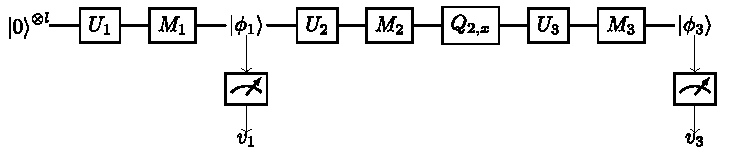
\includegraphics[width=\linewidth,height=0.78\textheight,keepaspectratio]{ccc2025-12-svg-03.pdf}\par

(a) Example of the process occurring in $\mathcal{Q}_{P}$ with $P=2$ and $Q=1$.


\par\noindent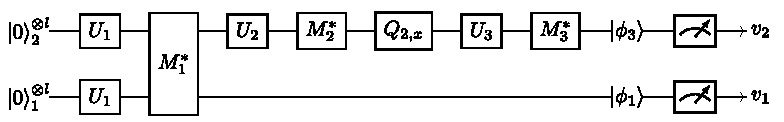
\includegraphics[width=\linewidth,height=0.78\textheight,keepaspectratio]{ccc2025-12-svg-04.pdf}\par

(b) The circuit $C^{*}$ in $\mathcal{Q}_{P}^{*}$ based on the example in \textbf{(a)}.


Figure 3: Examples of the quantum oracle model with non-collapsing measurements based on \textbf{(a)} Definition 11 and \textbf{(b)} Definition 13.



By using the definition above, we find that the query complexity of the two models is equivalent.\par



% SOURCE-ID Thmtheorem14


\par\medskip\noindent\textbf{
\textbf{Lemma 14}\textbf{.}
}\par



\emph{The query complexity of the original $\mathsf{PDQP}$ query model is equivalent to the query complexity of the adjusted $\mathsf{PDQP}$ query model.}\par



% END-SOURCE-ID Thmtheorem14




\par\medskip\noindent\textbf{Proof.}\par




Suppose that we query a circuit which performs $Q$ queries and $P$ non-collapsing measurements to the original oracle $\mathcal{Q}_{P}$. By our explanation of the query model above, we know that $\mathcal{Q}_{P}^{*}$ simulates the queries $Q_{i}$ by the query gate $Q_{i}^{*}$, obtaining the same query complexity.\par




On the other hand, suppose we have a circuit that is run by $\mathcal{Q}_{P}^{*}$. Each unitary $U^{*}_{i}$, measurement $M^{*}_{i}$ and query $Q^{*}_{i}$ may be run by the original oracle $\mathsf{PDQP}$ by only running the gates on the first register, leading to the same complexity.
$\blacktriangleleft$\par




We note that one obtains that the gate complexity of the models is equal in a similar way. Furthermore, it is important to mention that by going from $\mathcal{Q}_{P}$ to $\mathcal{Q}_{P}^{*}$ and vice-versa under the same input, we adjust the width of the circuits while maintaining equal depth. By the characterization of fidelity using Bhattacharyya coefficients [17], we know that fidelity between states may not decrease after measurement. We find that the same holds for our adjusted measurement gates, allowing us to restrict the power of $M^{*}$ in this model.\par



% SOURCE-ID Thmtheorem15


\par\medskip\noindent\textbf{
\textbf{Lemma 15}\textbf{.}
}\par



\emph{Let $(\rho^{\prime}_{1,i},\rho^{\prime}_{2,i})$ be the pair of states with different query oracles at step $i$ of $C^{*}$ before the application of $M^{*}_{i}$. Let $c\in\{1,2\}$ and $\rho_{c,i}=M^{*}_{i}\rho^{\prime}_{c,i}(M^{*}_{i})^{\dagger}$. Then,}\par


\[\begin{gathered}
\displaystyle F(\rho^{\prime}_{1,i},\rho^{\prime}_{2,i})\leq F(\rho_{1,i},\rho_{2,i})
\end{gathered}\]



% END-SOURCE-ID Thmtheorem15




\par\medskip\noindent\textbf{Proof.}\par




Let $c\in\{1,2\}$. The proof of the statement is done by explicitly defining the states $\rho^{\prime}_{c,i}$ as the sum of pure states whose purification results in the maximal fidelity, per Uhlmann’s theorem. We show that for any such purification, the same purification process increases the fidelity when applied to $\rho_{c,i}$. This lower-bounds $F(\rho_{1,i},\rho_{2,i})$ by Uhlmann’s theorem, proving our statement.\par




Let $k$ be an arbitrary integer. We define the state at each register the same due to the multiplicativity of fidelity.
As the gate $M^{*}_{i}$ only affects $r_{i}$ registers, we shall ignore the rest. Each of the $r_{i}$ registers is the following mixed state,\par


\[\begin{gathered}
\displaystyle\sigma_{c,i} \displaystyle=\sum_{k\in[k]}b_{c,k}\ket{\lambda_{c,k}}\bra{\lambda_{c,k}} \\
\displaystyle\ket{\lambda_{c,k}} \displaystyle=\sum_{j}\alpha_{c,j,k}\ket{j}_{\mathcal{M}}\ket{\chi_{c,j,k}}
\end{gathered}\]


where $b_{c,k}\in\mathbb{R}$, $\alpha_{c,j,k}\in\mathbb{C}$, $\mathcal{M}$ is the register being measured by $M_{i}^{*}$ and $\chi_{c,j,k}$ is its associated workspace.
The definition of $\ket{\lambda_{c,k}}$ in $\sigma_{c,i}$ is such that if we purify it as we do below, we obtain the maximum fidelity as shown by Uhlmann’s theorem.
Let $A=\otimes_{j}^{r_{i}}[k]_{j}$, $a\in A$ and $b^{*}_{c,a}=\prod_{r\in a}b_{c,r}$.
Therefore the entire state $\rho^{\prime}_{c,i}$ and its purification may be described as,\par




\[\begin{gathered}
\displaystyle\rho^{\prime}_{c,i} \displaystyle=\sigma_{c,i}^{\otimes r_{i}}=\sum_{a\in A}b^{*}_{c,a}(\otimes_{s\in a}\ket{\lambda_{c,s}}\bra{\lambda_{c,s}}) \\
\displaystyle\ket{\psi^{\prime}_{c,i}} \displaystyle=\sum_{a\in A}\sqrt{b^{*}_{c,a}}(\otimes_{s\in a}\ket{\lambda_{c,s}})\ket{s}
\end{gathered}\]


Let $a^{*}_{c,j,a}=\prod_{s\in A}\norm{\alpha_{c,j,s}}_{2}^{2}$, $d$ be the probability of measuring $j$ in $\sigma_{c,i}$, $d_{i,j}=\frac{1}{d^{r_{i}-1}}$ and $\alpha^{*}_{c,j,a}=\prod_{s\in A}\alpha_{c,j,s}$.
We apply $M^{*}_{i}$ to $\rho^{\prime}_{c,i}$, which adjusts the amplitudes and ensures that the register $\mathcal{M}$ measures to the same value $j$ over all $r_{i}$ registers. By using the definition of $M^{*}_{i}$ from Line 3,\par


\[\begin{gathered}
\displaystyle\rho_{c,i} \displaystyle=\sum_{a\in A,j}a^{*}_{c,j,a}d_{i,j}b^{*}_{c,a}(\otimes_{s\in a}\ket{\chi_{c,j,k}}\bra{\chi_{c,j,k}}) \\
\displaystyle\ket{\psi_{c,i}} \displaystyle=\sum_{a\in A,j}\alpha^{*}_{c,j,a}\sqrt{d_{i,j}b^{*}_{c,a}}(\otimes_{s\in a}\ket{\chi_{c,j,k}})\ket{s}
\end{gathered}\]


By using our assumption about $\rho^{\prime}_{c,i}$, we find,\par


\[\begin{gathered}
\displaystyle F(\rho^{\prime}_{1,i},\rho^{\prime}_{2,i}) \displaystyle=\bra{\psi^{\prime}_{1,i}}\ket{\psi^{\prime}_{2,i}} \\
\displaystyle=\sum_{\begin{subarray}{c}a_{1}\in A_{1}\\
a_{2}\in A_{2}\end{subarray}}\sqrt{b^{*}_{1,a_{1}}b^{*}_{2,a_{2}}}\prod_{\begin{subarray}{c}s_{1}\in a_{1}\\
s_{2}\in a_{2}\end{subarray}}\bra{\lambda_{1,s_{1}}}\ket{\lambda_{2,s_{2}}}\delta_{s_{1},s_{2}} \\
\displaystyle=\sum_{a\in A,j}\sqrt{b^{*}_{1,a}b^{*}_{2,a}}\prod_{s\in a}\bra{\chi_{1,j,s}}\ket{\chi_{2,j,s}}\alpha_{1,j,s}\alpha_{2,j,s} \\
\displaystyle\leq\sum_{a\in A,j}\sqrt{b^{*}_{1,a}b^{*}_{2,a}}\alpha^{*}_{1,j,a}\alpha^{*}_{2,j,a}d_{i,j}\prod_{s\in a}\bra{\chi_{1,j,s}}\ket{\chi_{2,j,s}} \\
\displaystyle=\bra{\psi_{1,i}}\ket{\psi_{2,i}} \\
\displaystyle\leq\bra{\psi^{max}_{1,i}}\ket{\psi^{max}_{2,i}} \\
\displaystyle=F(\rho_{1,i},\rho_{2,i})
\end{gathered}\]


Lines 5- 7 are by our definitions above, Line 8 follows as $d_{i,j}\geq 1$, and Line 10 follows by Uhlmann’s theorem where we define $(\psi^{max}_{1,i},\psi^{max}_{2,i})$ as the pair of purifications which maximize $F(\rho_{1,i},\rho_{2,i})$.
$\blacktriangleleft$\par






\par\medskip\noindent\textbf{
4 Lower-bounds on non-collapsing measurements}\par




In this section we expand the bounds established in [5]. First, we generalize their lower-bound to a wider selection of problems. Next, we show that the $\tilde{O}(N^{1/3})$ search algorithm from [5] is optimal up to logarithmic factors by obtaining a $\Omega(N^{1/3})$ lower-bound.\par




\par\medskip\noindent\textbf{
4.1 Weighted adversary method}\par




Our proof closely follows the original proof of the positive-weighted adversary method [8]. There are two main adjustments. We employ Lemma 15 to argue that using partial measurements won’t affect the progress measure. Additionally, we consider the effect of non-collapsing measurements by using the model in Definition 13. In order to accommodate the second change, we will require the following Proposition.\par



% SOURCE-ID Thmtheorem16


\par\medskip\noindent\textbf{
\textbf{Proposition 16}\textbf{.}
}\par



\emph{For any $k\in\mathbb{N}$ and $r,s\in\mathbb{R}$ where $0\leq r\leq 1$ and $0\leq s\leq 2r$,}\par


\[\begin{gathered}
\displaystyle ks\geq r^{k}-(r-s)^{k}
\end{gathered}\]



% END-SOURCE-ID Thmtheorem16



\par\medskip\noindent\textbf{Proof.}\par




Let $A_{k,s}=ks-r^{k}+(r-s)^{k}$. Note that the statement holds when $k=1$. Therefore let $k\geq 2$.\par




Assume $s\leq r$. We have,\par


\[\begin{gathered}
\displaystyle A_{n+1,s}-A_{n,s} \displaystyle=s-r^{n}(r-1)+(r-s)^{n}(r-s-1) \\
\displaystyle=s-r^{n}s+r^{n}s-r^{n}(r-1)+(r-s)^{n}(r-s-1) \\
\displaystyle=s(1-r^{n})+((r-s)^{n}-r^{n})(r-1-s)
\end{gathered}\]


By the bounds on $r,s$ and the assumption that $s\leq r$, we have that $s(1-r^{n})\geq 0$, $(r-1-s)\leq 0$ and $((r-s)^{n}-r^{n})\leq 0$. As $A_{n+1,s}-A_{n,s}\geq 0$, the statement holds.\par




Assume $s>r$. Additionally, without loss of generality, assume $k$ is odd. We find,\par


\[\begin{gathered}
\displaystyle A_{k,s} \displaystyle=ks-(r^{k}-(r-s)^{k}) \\
\displaystyle\geq ks-(r^{k}-(r-2r)^{k}) \\
\displaystyle=ks-2r^{k}
\end{gathered}\]


As $k\geq 2$ and $s>r$, $A_{k,s}\geq 0$.
$\blacktriangleleft$\par




We define the progress measure as,\par


\[\begin{gathered}
\displaystyle\Phi(t)=\sum_{(x,y)\in R}w(x,y)F(\rho_{x,t},\rho_{y,t})
\end{gathered}\]




We bound the progress made at each step using the following lemma.\par



% SOURCE-ID Thmtheorem17


\par\medskip\noindent\textbf{
\textbf{Lemma 17}\textbf{.}
}\par



\emph{Let $f$ be a boolean function with a valid weight scheme and its associated maximum load $v_{max}$. Then the progress made by a $\mathsf{PDQP}$ algorithm each query $t\in[Q]$ is bounded by,}\par


\[\begin{gathered}
\displaystyle\Phi(t-1)-\Phi(t)\leq P\,v_{max}\Phi(0)
\end{gathered}\]



% END-SOURCE-ID Thmtheorem17




\par\medskip\noindent\textbf{Proof.}\par




By the unitary invariance of fidelity, we will ignore the application of unitaries. Similarly, by Lemma 15, we won’t consider partial measurements as their effect may not decrease the progress measure. Therefore, without loss of generality, we assume our states are always pure. Additionally, we assume that during query $t$, we have $D$ non-collapsing measurements left and have already performed $d=P-D$.\par




Let $\ket{\psi_{x,t}}$ denote the state of the algorithm on input $x$ at query $t$ and $\ket{\psi_{x,t}^{\prime}}$ denote the same before the application of the oracle. Additionally, let $\ket{\psi_{x,t}^{*}}$ be the state during query $i$ of $C^{*}$ as defined in Definition 13, while $\ket{\psi_{x,t}^{\prime*}}$ is the state in $C^{*}$ before the query. Using these definitions, we obtain the following identity,\par


\[\begin{gathered}
\displaystyle\Phi(t-1)-\Phi(t) \displaystyle=\sum_{(x,y)\in R}w(x,y)F(\psi_{x,t-1}^{*},\psi_{y,t-1}^{*})-\sum_{(x,y)\in R}w(x,y)F(\psi_{x,t}^{*},\psi_{y,t}^{*}) \\
\displaystyle\leq\sum_{(x,y)\in R}w(x,y)\absolutevalue{\bra{\psi_{x,t-1}^{*}}\ket{\psi_{y,t-1}^{*}}-\bra{\psi_{x,t}^{*}}\ket{\psi_{y,t}^{*}}} \\
\displaystyle=\sum_{(x,y)\in R}w(x,y)\absolutevalue{\bra{\psi_{x,t}^{\prime*}}\ket{\psi_{y,t}^{\prime*}}-\bra{\psi_{x,t}^{*}}\ket{\psi_{y,t}^{*}}}
\end{gathered}\]




Let $\ket{\psi_{x,t}}=\sum_{i}\alpha_{x,i}\ket{i}_{\mathcal{Q}}\ket{\phi_{x,i}}_{\mathcal{W}}$ where $\mathcal{Q}$ is the query register and $\mathcal{W}$ is the workspace register associated with that query register. As we have $D$ non-collapsing measurements left to perform, an oracle call will affect the $D$ copies of the state labeled by $\mathcal{O}$ and neglect the remaining $d$.\par


\[\begin{gathered}
\displaystyle\ket{\psi_{x,t}^{*}}=\ket{\psi_{x,1}}\otimes..\otimes\ket{\psi_{x,d}}\otimes(\ket{\psi_{x,t}}_{\mathcal{O}})^{\otimes D}
\end{gathered}\]




For the sake of simplicity, let,\par


\[\begin{gathered}
\displaystyle\hat{S}_{i} \displaystyle=\sum_{i}\alpha_{x,i}\alpha_{y,i}\bra{\phi_{x,i}}\ket{\phi_{y,i}} \\
\displaystyle\hat{S}_{x(i)=y(i)} \displaystyle=\sum_{i:x(i)=y(i)}\alpha_{x,i}\alpha_{y,i}\bra{\phi_{x,i}}\ket{\phi_{y,i}} \\
\displaystyle\hat{k} \displaystyle=\sum_{i:x(i)\neq y(i)}\alpha_{x,i}\alpha_{y,i}\bra{\phi_{x,i}}\ket{\phi_{y,i}}
\end{gathered}\]


We find that,\par


\[\begin{gathered}
\displaystyle\Phi(t-1)-\Phi(t)\leq \displaystyle\sum_{(x,y)\in R}w(x,y)\left|\bra{\psi_{x,t}^{\prime*}}\ket{\psi_{y,t}^{\prime*}}-\bra{\psi_{x,t}^{*}}\ket{\psi_{y,t}^{*}}\right| \\
\displaystyle= \displaystyle\sum_{(x,y)\in R}w(x,y)\absolutevalue{\bra{\phi_{x,1}}\ket{\phi_{y,1}}...\bra{\phi_{x,d}}\ket{\phi_{y,d}}} \\
\displaystyle\qquad\absolutevalue{\hat{S}_{i_{1}}..\hat{S}_{i_{D}}-\left(\hat{S}_{x(i_{1})=y(i_{1})}-\hat{k}_{1}\right)...\left(\hat{S}_{x(i_{D})=y(i_{D})}-\hat{k}_{D}\right)} \\
\displaystyle\leq \displaystyle\sum_{(x,y)\in R}w(x,y)\absolutevalue{\hat{S}_{i}^{D}-\left(\hat{S}_{i}-2\hat{k}\right)^{D}} \\
\displaystyle\leq \displaystyle\sum_{(x,y)\in R}2w(x,y)D\hat{k} \\
\displaystyle= \displaystyle D\sum_{\begin{subarray}{c}(x,y)\in R\\
i:x(i)\neq y(i)\end{subarray}}2w(x,y)\left|\alpha_{x,i}\right|\left|\alpha_{y,i}\right| \\
\displaystyle\leq \displaystyle P\;v_{max}\Phi(0)
\end{gathered}\]


Line 15 was shown on Line 14, Line 16 uses the multiplicativity of fidelity, Line 17 holds as the inner product of two states is bounded by 1, Line 18 uses Proposition 16 by setting $r=\hat{S}_{i}$ and $s=2\hat{k}$, and Line 20 is by Proposition 10 and $D\leq P$.
$\blacktriangleleft$\par




Lemma 17 is sufficient to obtain the bound below.\par



% SOURCE-ID Thmtheorem18


\par\medskip\noindent\textbf{
\textbf{Lemma 18}\textbf{.}
}\par



\emph{Let $f$ be a boolean function with a weight scheme and its associated maximum load $v_{max}$. In a $\mathsf{PDQP}$ setting, the following holds,}\par


\[\begin{gathered}
\displaystyle QP=\Omega\left(\frac{1}{v_{max}}\right)
\end{gathered}\]



% END-SOURCE-ID Thmtheorem18




\par\medskip\noindent\textbf{Proof.}\par




Assuming success probability of $1-\epsilon$, we have that $\Phi(T)\leq 2\sqrt{\epsilon(1-\epsilon)}\Phi(0)$. By Lemma 17,\par


\[\begin{gathered}
\displaystyle Q\geq\frac{\Phi(0)-\Phi(T)}{\Phi(t-1)-\Phi(t)}\geq\frac{1-2\sqrt{\epsilon(1-\epsilon)}}{Pv_{max}}
\end{gathered}\]


$\blacktriangleleft$\par






\par\medskip\noindent\textbf{
4.2 Lower-bound on search}\par




We use the proof of a $\Omega(N^{1/3})$ lower-bound on $\mathsf{PDQP}$ without collapsing measurements from [5] and apply Lemma 15 in order to introduce partial measurement.\par



% SOURCE-ID Thmtheorem19


\par\medskip\noindent\textbf{
\textbf{Lemma 19}\textbf{.}
}\par



\emph{Any algorithm solving the search problem in $\mathsf{PDQP}$ setting using $Q$ queries and and $P$ non-collapsing measurements satisfies,}\par


\[\begin{gathered}
\displaystyle Q+P=\Omega(N^{1/3})
\end{gathered}\]



% END-SOURCE-ID Thmtheorem19



\par\medskip\noindent\textbf{Proof.}\par




Consider a $\mathsf{PDQP}$ algorithm where $Q=P=o(N^{1/3})$. We compare the cases when there are no marked items versus when $x$ is a marked item. Let their respective quantum states at step $t$ be $\rho_{t},\rho_{t}^{x}$ and $\psi_{t}$ and $\psi_{t}^{x}$ be states of the same algorithm without partial measurement. By Lemma 7, we have,\par


\[\begin{gathered}
\displaystyle\sum_{x}\norm{\psi_{t}-\psi_{t}^{x}}^{2}_{2}\leq 4Q^{2}
\end{gathered}\]




By summing over $P$ non-collapsing measurements and using an averaging argument, there exists an $x$ such that,\par


\[\begin{gathered}
\displaystyle\sum_{t}\norm{\psi_{t}-\psi_{t}^{x}}^{2}_{2}\leq\frac{4PQ^{2}}{N}
\end{gathered}\]




By our assumption on the number of queries, this norm must be constant. Let’s say that $\norm{\psi_{t}-\psi_{t}^{x}}_{2}^{2}\leq 0.01$. Let $\Phi=\otimes_{t}\rho_{t}$ represent all the states before measurement and $V$ the distribution of their measurements. In order to notice the presence of a marked item, we require $|V-V_{x}|_{1}\geq\Omega(1)$. Therefore,\par


\[\begin{gathered}
\displaystyle\Omega(1)\leq|V-V_{x}|_{1} \displaystyle\leq\norm{\Phi-\Phi_{x}} \\
\displaystyle\leq\sqrt{1-F(\Phi,\Phi_{x})^{2}} \\
\displaystyle=\sqrt{1-|\Pi_{t}F(\rho_{t},\rho_{t}^{x})|^{2}} \\
\displaystyle\leq\sqrt{1-|\Pi_{t}\bra{\psi_{t}}\ket{\psi_{t}^{x}}|^{2}} \\
\displaystyle\leq\sqrt{1-\Pi_{t}e^{-\norm{\psi_{t}-\psi_{t}^{x}}^{2}_{2}}} \\
\displaystyle\leq\sqrt{1-e^{-\frac{4PQ^{2}}{N}}} \\
\displaystyle=o(1)
\end{gathered}\]




Line 22 follows by the definition of trace norm, Line 24 holds as by Lemma 15, we may assume we did not perform partial measurements, and Line 25 uses the inequality\par


\[\begin{gathered}
\displaystyle|\bra{\psi_{t}}\ket{\psi_{t}^{x}}|\geq\text{Re}(\bra{\psi_{t}}\ket{\psi_{t}^{x}})\geq e^{-\norm{\psi_{t}-\psi_{t}^{x}}^{2}_{2}}
\end{gathered}\]


which holds as $1-x\geq e^{-2x}$ when $0\leq x\leq 0.01$.
$\blacktriangleleft$\par







\par\medskip\noindent\textbf{
5 Non-collapsing measurements and non-adaptive queries}\par




\par\medskip\noindent\textbf{
5.1 Non-adaptive query model}\par




In this section, we describe the non-adaptive query model and prove its lower-bounds. Informally, the model performs all of its queries at the start of the computation, meaning that they are independent of the input $x$. We obtain a trade-off between $Q$ and $P$.\par




The notation and proof closely follows that of [23]. Assume we perform $Q$ non-adaptive queries. Given an oracle operator $O_{x}$ for an input $x$, we define the query as,\par


\[\begin{gathered}
\displaystyle O_{x}^{Q}\ket{i_{1},b_{1},...i_{Q},b_{Q}}\rightarrow(-1)^{s}\ket{i_{1},b_{1},...i_{Q},b_{Q}}
\end{gathered}\]




where $s=\sum_{j\in[Q]}x(i_{j})\cdot b_{j}$. The algorithm may be described as follows,\par


\[\begin{gathered}
\displaystyle M_{P}U_{P}...M_{1}U_{1}O_{x}^{Q}U_{0}\ket{0}
\end{gathered}\]




Assume we perform a non-collapsing measurement after every unitary except $U_{0}$. The label $nq$ describes a variable in the non-adaptive query setting. For example, $P^{nq}$ describes the number of non-collapsing measurements performed. Next, we define a variation of the weight scheme from Definition 8 for non-adaptive queries. The main idea of the proof is lower-bounding the minimum size of the initial parallel query by arguing that a smaller query would require at least two rounds of parallel queries. We use the superscript $k$ to denote a variable for the parallel query of size $k\in\mathbb{N}$.\par



% SOURCE-ID Thmtheorem20


\par\medskip\noindent\textbf{
\textbf{Definition 20}\textbf{ }(Weight scheme of [23])\textbf{.}
}\par



\emph{Consider an arbitrary boolean function $f$ and an input $x$. We define ${}^{k}x=x^{k}$, ${}^{k}f({}^{k}x)=f(x)$ and an index-tuple $I=(i_{1},...i_{k})$. Therefore $x(I)=(x(i_{1}),...,x(i_{k}))$.}\par




\emph{Let $w,wt$ and $v$ be the weight variables as in Definition 8 for $f$. Then $W,WT$ and $V$ are their variations for ${}^{k}f$. We let $W({}^{k}x,{}^{k}y)=w(x,y)$.}\par



% END-SOURCE-ID Thmtheorem20



We will use the following lemma from [23],\par



% SOURCE-ID Thmtheorem21


\par\medskip\noindent\textbf{
\textbf{Lemma 21}\textbf{ }(Lemma 2 in [23])\textbf{.}
}\par



\emph{Let $x$ be an input and $w$ a weight function. For any $k\in\mathbb{N}$ and an index-tuple $I=(i_{1},..,i_{k})$,}\par


\[\begin{gathered}
\displaystyle\frac{WT({}^{k}x)}{V({}^{k}x,I)}\geq\frac{1}{k}\min_{j\in[k]}\frac{wt(x)}{v(x,i_{j})}
\end{gathered}\]



% END-SOURCE-ID Thmtheorem21




\par\medskip\noindent\textbf{
5.2 Weighted adversary method with non-adaptive queries}\par




We prove the results on non-adaptive queries using the technique from [23], resulting in the lemma below.\par



% SOURCE-ID Thmtheorem22


\par\medskip\noindent\textbf{
\textbf{Lemma 22}\textbf{.}
}\par



\emph{Consider a function $f$ with a weight scheme $w$. Then any $\mathsf{PDQP}^{nq}$ algorithm with $Q$ queries and $P$ non-adaptive measurements satisfies,}\par


\[\begin{gathered}
\displaystyle QP=\Omega\left(\max_{w}\max_{s\in\{0,1\}}\min_{\begin{subarray}{c}x,i\\
f(x)=s\end{subarray}}\frac{wt(x)}{v(x,i)}\right)
\end{gathered}\]



% END-SOURCE-ID Thmtheorem22



In order to establish Lemma 22, we will first establish the following result which connects Lemma 18 and weights for non-adaptive inputs.\par



% SOURCE-ID Thmtheorem23


\par\medskip\noindent\textbf{
\textbf{Lemma 23}\textbf{.}
}\par



\emph{Let $w$ be a weight function for $f$. Then $W$ is a valid weight function for ${}^{k}f$ and any algorithm solving ${}^{k}f$ using $Q$ queries and $P$ non-collapsing measurements satisfies,}\par


\[\begin{gathered}
\displaystyle QP\geq C_{\epsilon}\min_{{}^{k}x,{}^{y}x,I}\left(\frac{WT({}^{k}x)WT({}^{k}y)}{V({}^{k}x,I)V({}^{k}y,I)}\right)^{1/2}
\end{gathered}\]


\emph{where $C_{\epsilon}=\sqrt{\frac{1-2\sqrt{\epsilon(1-\epsilon)}}{2}}$.}\par



% END-SOURCE-ID Thmtheorem23



\par\medskip\noindent\textbf{Proof.}\par




By Definition 20, as $W({}^{k}x,{}^{k}y)=w(x,y)$, we may apply Lemma 18 to obtain the bound.
$\blacktriangleleft$\par




We will prove the following lemma:\par




% SOURCE-ID Thmtheorem24


\par\medskip\noindent\textbf{
\textbf{Lemma 24}\textbf{.}
}\par



\emph{Let $w$ be a valid weight function and $x,y$ such that $f(x)\neq f(y)$. Then,}\par


\[\begin{gathered}
\displaystyle Q^{nq}P^{nq}\geq C^{2}_{\epsilon}\min_{x,y}\;\max\;\left(\min_{i}\frac{wt(x)}{v(y,i)},\min_{i}\frac{wt(y)}{v(x,i)}\right)
\end{gathered}\]



% END-SOURCE-ID Thmtheorem24





\par\medskip\noindent\textbf{Proof.}\par




Let $k\in\mathbb{N}$ be such that\par


\[\begin{gathered}
\displaystyle k<C^{2}_{\epsilon}\min_{x,y}\max\left(\min_{i}\frac{wt(x)}{v(x,i)},\min_{i}\frac{wt(y)}{v(y,i)}\right)
\end{gathered}\]


We shall show that performing $k$ non-adaptive queries would require us to repeat the computation more than once, implying that $Q^{nq}P^{nq}>k$. By using Lemma 21 and the fact that $WT({}^{k}x)\geq V({}^{k}x,I)$ for any $x$ and $I$, we have that,\par


\[\begin{gathered}
\displaystyle\frac{WT({}^{k}x)}{V({}^{k}x,I)}\frac{WT({}^{k}y)}{V({}^{k}y,I)} \displaystyle\geq\max\left(\frac{WT({}^{k}x)}{V({}^{k}x,I)},\frac{WT({}^{k}y)}{V({}^{k}y,I)}\right) \\
\displaystyle\geq\frac{1}{k}\max\left(\min_{j\in[k]}\frac{wt(x)}{v(x,i_{j})},\min_{l\in[k]}\frac{wt(y)}{v(y,i_{l})}\right)
\end{gathered}\]


Therefore we have that,\par


\[\begin{gathered}
\displaystyle\min_{{}^{k}x,{}^{k}y,I}\frac{WT({}^{k}x)}{V({}^{k}x,I)}\frac{WT({}^{k}y)}{V({}^{k}y,I)} \displaystyle\geq\frac{1}{k}\min_{{}^{k}x,{}^{k}y,I}\max\left(\min_{j\in[k]}\frac{wt(x)}{v(x,i_{j})},\min_{l\in[k]}\frac{wt(y)}{v(y,i_{l})}\right) \\
\displaystyle\geq\frac{1}{k}\min_{x,y}\max\left(\min_{i}\frac{wt(x)}{v(x,i)},\min_{i}\frac{wt(y)}{v(y,i)}\right) \\
\displaystyle\geq\frac{1}{C^{2}_{\epsilon}}
\end{gathered}\]


Where we applied our assumption on $k$. Therefore according to Lemma 23, $Q^{nq}P^{nq}>1$, proving the lemma.
$\blacktriangleleft$\par




Lemma 24 directly implies Lemma 22.\par







\par\medskip\noindent\textbf{
6 Lower-bounding quantum computation with copies}\par




In this section, we apply the ideas from Lemma 18 to $\mathsf{CBQP}$, quantum computation which is able to create a copy of any state. Another way to consider $\mathsf{CBQP}$ is as the computational class representing a world where the no-cloning theorem does not hold. The point of this section is to explicitly showcase the power difference between non-collapsing measurements and copying a state. As most steps in our analysis are identical, we only focus on the differences.\par




\par\medskip\noindent\textbf{
6.1 Computational model with copies}\par




The key difference between $\mathsf{PDQP}$ and $\mathsf{CBQP}$ is that the latter has the ability to apply unitaries to the copies after creating them, while $\mathsf{PDQP}$ must immediately collapse them. As these copies may become entangled, purifying the algorithm in a similar manner as in Definition 13, meaning explicitly creating copies of each state in order to analyze it, will require additional registers. Therefore, as we explain below, instead of using $O(P)$ registers as in $\mathsf{PDQP}$, we will need $O(2^{P})$ registers.\footnote{$P$ denotes either the number of non-collapsing measurements or copies. This will be obvious from context.}\par





\par\noindent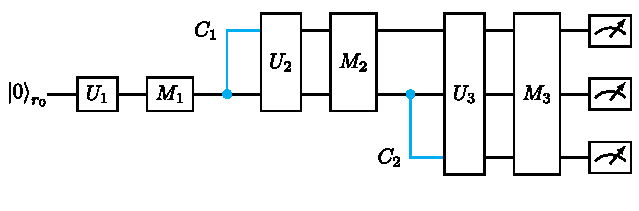
\includegraphics[width=\linewidth,height=0.78\textheight,keepaspectratio]{ccc2025-12-svg-05.pdf}\par

(a) Example of a $\mathsf{CBQP}$ circuit. The cyan wires signify a copy operation.


\par\noindent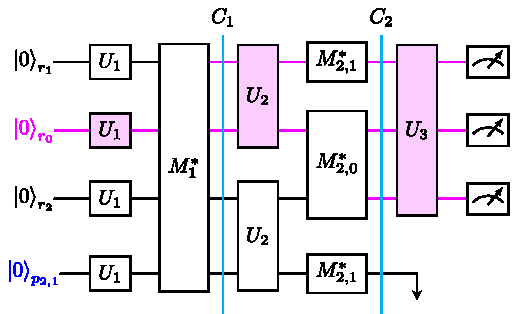
\includegraphics[width=\linewidth,height=0.78\textheight,keepaspectratio]{ccc2025-12-svg-06.pdf}\par

(b) A purified version of the circuit above. The magenta register and wires are the same as in the circuit above, while the blue register is only to assist in the creation of a perfect copy and is not part of the original circuit above. Note that the gate $M^{*}_{2,1}$ is over registers $r_{1}$ and $p_{2,1}$.


Figure 4: Example of purifying a $\mathsf{CBQP}$ circuit.



Assume we perform $P$ copies in total. Let $r_{0}$ be the starting register and for $i>0$, $r_{i}$ be its copies at step $i$. Without loss of generality, assume we only copy and apply the oracle to $r_{0}$. The gate $C_{i}$ symbolizes a copy gate, which creates a copy, allowing us to apply unitaries across all registers $r_{j}$ for $j\leq i$. Prior to applying the $C_{i}$ gate, we must ensure that $r_{i}$ and $r_{0}$ are copies, meaning that similarly to Definition 13, we apply unitary $U$ in parallel to both. Finally, we account for the effect of partial measurement by using a partial measurement gate $M^{*}_{j}$, ensuring that partial measurement results before applying $C_{i}$ are the same across all registers. When adding queries to this model, we follow the same steps as in Definition 13.\par




Finally, as each copy must mimic the register it is copying, we need to add further purification registers $p_{i,j}$ for each copy $i$. These registers mimic the process of the register until it has been copied. As each copy may be entangled, with each additional copy, the amount of purification registers doubles. In order to describe copy $i$ of the computation, we require $2^{i}$ registers including the register $r_{i}$. Therefore the total number of registers is $r^{P}$. An example of a circuit with the ability to copy and its purification is in Figure 4.\par





\par\medskip\noindent\textbf{
6.2 Adversary lower-bound}\par




We prove a version of Lemma 17 for $\mathsf{CBQP}$.\par



% SOURCE-ID Thmtheorem25


\par\medskip\noindent\textbf{
\textbf{Lemma 25}\textbf{.}
}\par



\emph{Let $f$ be a boolean function with a valid weight scheme and its associated maximum load $v_{max}$ as in Definition 9. Then the progress made by a $\mathsf{CBQP}$ algorithm each query $t$ is bounded by,}\par


\[\begin{gathered}
\displaystyle\Phi(t-1)-\Phi(t)\leq 2^{P}v_{max}\Phi(0)
\end{gathered}\]


\emph{where $P$ is the number of copies.}\par



% END-SOURCE-ID Thmtheorem25



\par\medskip\noindent\textbf{Proof.}\par




First, we shall ignore the effect of unitaries and partial measurement by the same arguments and definitions of variables as in Lemma 17. In this case $D\leq 2^{P}$. We obtain the following result,\par


\[\begin{gathered}
\displaystyle\Phi(t-1)-\Phi(t)\leq \displaystyle\sum_{(x,y)\in R}w(x,y)\absolutevalue{\bra{\psi_{x,t}^{\prime*}}\ket{\psi_{y,t}^{\prime*}}-\bra{\psi_{x,t}^{*}}\ket{\psi_{y,t}^{*}}} \\
\displaystyle\leq \displaystyle\sum_{(x,y)\in R}w(x,y)\absolutevalue{\hat{S}_{i}^{D}-\left(\hat{S}_{i}-2\hat{k}\right)^{D}} \\
\displaystyle\leq \displaystyle 2^{P}v_{max}\Phi(0)
\end{gathered}\]


$\blacktriangleleft$\par




We find the following relationship between the number of queries and copies.\par



% SOURCE-ID Thmtheorem26


\par\medskip\noindent\textbf{
\textbf{Lemma 26}\textbf{.}
}\par



\emph{Let $f$ be a boolean function with a weight scheme and its associated maximum load $v_{max}$. A $\mathsf{CBQP}$ algorithm with $Q$ queries and $P$ copies satisfies,}\par


\[\begin{gathered}
\displaystyle Q2^{P}=\Omega\left(\frac{1}{v_{max}}\right)
\end{gathered}\]



% END-SOURCE-ID Thmtheorem26



Lemma 26 implies that the algorithm in [9] to solve search is optimal and explains the discrepancy between $\mathsf{CBQP}$ and $\mathsf{PDQP}$.\par







\par\medskip\noindent\textbf{
7 Bounds on problems with non-collapsing measurements}\par




\par\medskip\noindent\textbf{
7.1 Proofs of applications of the lower-bounding techniques}\par




We shall apply Lemmata 18 and 24 on concrete problems in order to compare the two models. First, let us note that the positive-weighted adversary technique may be reduced to the basic adversary technique by setting the weights $w(x,y)$ to 1.\par



% SOURCE-ID Thmtheorem27


\par\medskip\noindent\textbf{
\textbf{Corollary 27}\textbf{.}
}\par



\emph{Let $f:\{0,1\}^{n}\rightarrow\{0,1\}$ be a boolean function, $X,Y$ be two subsets of $1$-inputs and $0$-inputs respectively and $R$ a relation $R\subseteq X\times Y$. Furthermore, let $m,m^{\prime},l,l^{\prime}$ be the same as in Result 1. Then a $\mathsf{PDQP}$ query algorithm solving $f$ with $Q$ queries and $P$ non-collapsing measurements satisfies,}\par


\[\begin{gathered}
\displaystyle QP=\Omega\left(\sqrt{\frac{mm^{\prime}}{ll^{\prime}}}\right)
\end{gathered}\]


\emph{Furthermore, a $\mathsf{PDQP}$ query algorithm with non-adaptive queries solving $f$ with $Q^{nq}$ queries and $P^{nq}$ non-collapsing measurements satisfies,}\par


\[\begin{gathered}
\displaystyle Q^{nq}P^{nq}=\Omega\left(\max\left\{\frac{m}{l},\frac{m^{\prime}}{l^{\prime}}\right\}\right)
\end{gathered}\]



% END-SOURCE-ID Thmtheorem27



\par\medskip\noindent\textbf{Proof.}\par




In both Lemmata 18 and 24, let $w(x,y)=1$. Then $w(x)\geq m$ or $m^{\prime}$ and $v(x,i)\leq l$ or $l^{\prime}$ depending on whether $x\in X$ or $x\in Y$.
$\blacktriangleleft$\par




Let us obtain the values $m,m^{\prime},l,l^{\prime}$ for the search, majority, collision and element distinctness problems. For each problem, we shall define the sets $X,Y$ and their relation $R$ which maximizes $m,m^{\prime}$ while minimizing $l,l^{\prime}$. In addition to that, we also describe their algorithm. As has been done during the entirety of the document, we let $N$ be the size of the input. Finally, we note that a summary of the results described below may be found in Table 1.\par





\par\medskip\noindent\textbf{Search problem.}\par




We know that the query complexity of the search problem in $\mathsf{PDQP}$ is $\tilde{\Theta}(N^{1/3})$ due to the algorithm in [5], while our Lemma 19 proves that this algorithm is tight up to logarithmic factors. However, the same technique does not apply to $\mathsf{PDQP}$ with non-adaptive queries. We may split the inputs for search as follows:\par


\begin{itemize}


\item[] 
$\blacksquare$ 


Let $X=\{0\}$ as $f(x)=0$ if and only if $x=0$.\par





\item[] 
$\blacksquare$ 


Let $Y=\{y:|y|=1\}$ as these are the only values which only differ by 1 character from any input in $X$.\par





\end{itemize}




Therefore we find that $m=N$ as we may choose any index $i\in[N]$ to go from $X$ to $Y$. Furthermore, $m^{\prime}=l=l^{\prime}=1$ as each of these connections between $X$ and $Y$ only occur on one index. By Corollary 27, the query complexity of the search problem in the $\mathsf{PDQP}$ setting with non-adaptive measurements is $\Omega(\sqrt{N})$. This is tight as one may run an algorithm where we partition $[N]$ into $\sqrt{N}$ sets and query each separately. Afterwards, we may perform non-collapsing measurements on all partitions at once which, with $\tilde{O}(\sqrt{N})$ would return a marked item with high probability if there exists one.\par





\par\medskip\noindent\textbf{Majority problem.}\par




To lower-bound the query complexity of the majority problem, we shall split the sets $X$ and $Y$ ones whose Hamming weight differs by one. Due to the structure of the problem, this is only possible when the Hamming weight is around $N/2$. Therefore let $X=\{x:|x|=N/2\}$, $Y:\{y:|y|=N/2+1\}$ and $(x,y)\in R$ if and only if $|\{x(i):x(i)\neq y(i)\}|=1$. This means that $m=N/2$, $m^{\prime}=N/2+1$ and $l=l^{\prime}=1$. Therefore, by Corollary 27, the lower-bounds for $\mathsf{PDQP}$ is $\Omega(\sqrt{N})$ in both $\mathsf{PDQP}$ cases, regardless of the adaptivity of queries.\par




Similarly to the non-adaptive algorithm for search, the best algorithm for the problem is performing $\sqrt{N}$ queries partitions of the input, each of size $\sqrt{N}$. Afterwards, we may perform $\tilde{O}(\sqrt{N})$ non-collapsing measurements. By the coupon collector’s problem, we will obtain all values with high probability, meaning the complexity of the problem is $\tilde{O}(\sqrt{N})$.\par





\par\medskip\noindent\textbf{Element Distinctness problem.}\par




To analyze the element distinctness problem, we let $X$ be the set of injective functions and $Y$ the set of functions which are almost injective. By almost injective, we mean that there exists exactly one pair of inputs $(x,x^{\prime})$ such that $f(x)=f(x^{\prime})$. Then we may define the relation between these sets of inputs as those which only require one change of outputs. Explicitly, $(f,f^{\prime})\in R$ if and only if $|\{x:f(x)\neq f^{\prime}(x)\}|=1$. Thus every injective function may become almost injective by changing any one of its image to another image which already has a preimage. Therefore $m=N$ and $l=1$. On the other hand, one may only choose one of two indices if they want to turn an almost injective function into an injective function by changing a single index. Therefore $m^{\prime}=2$ and $l^{\prime}=1$. Thus we find that the element distinctness problem in the $\mathsf{PDQP}$ query models with and without adaptive queries have a $\Omega(N^{1/4})$ and $\Omega(\sqrt{N})$ lower-bound respectively. Finally, the algorithm is the same as for non-adaptive search and the majority problem, giving us a query bound of $\tilde{O}(\sqrt{N})$.\par






\par\medskip\noindent\textbf{
7.2 Polynomial method lower-bounding technique}\par




We applied a $\mathsf{BQP}$ lower-bounding technique to $\mathsf{PDQP}$, but it is not tight in all situations. This may be due to the fact that the lower-bound establishes a $QP$ relationship instead of $Q+P$. We note that the lower-bound on search in [5] had the same issue. It would be interesting if one was able to apply the polynomial method to the setting. One approach towards this would be going in the spirit of Definition 13. Let $p_{i}(x)$ be the polynomial associated with the amplitudes of the state at register $i$. One may attempt to restrict each $p_{i}(x)$ in two ways. First, for each $i$, one would ensure that $p_{i}(x)$ builds on $p_{i-1}(x)$ in that if we omitted the last query from $p_{i}(x)$, we would obtain $p_{i-1}(x)$. Second, the polynomial $p(x)$ describing the amplitude of the entire state is a product of all $p_{i}(x)$ with a caveat. Without partial measurement, $p(x)=\prod_{i}p_{i}(x)$. However, after partial measurement, $p_{i}(x)$ would become the sum of several polynomials, $p_{i}(x)=\sum_{j}p_{i}^{j}(x)$ where the superscript $j$ signals a measurement result. In order to ensure partial measurement remains consistent along all polynomials, we would require $p(x)=\sum_{j}\prod_{i}p_{i}^{j}(x)$. We note that a list of other open problems we found interesting may be found in Subsection 1.5.\par






\par\medskip\noindent\textbf{References}\par



\begin{itemize}


\item[] 
[1]

Scott Aaronson.


Quantum computing and hidden variables ii: The complexity of sampling
histories, 2004.


arXiv:quant-ph/0408119.





\item[] 
[2]

Scott Aaronson.


Quantum computing, postselection, and probabilistic polynomial-time,
2004.


arXiv:quant-ph/0412187.





\item[] 
[3]

Scott Aaronson.


Impossibility of succinct quantum proofs for collision-freeness,
2011.


arXiv:1101.0403.





\item[] 
[4]

Scott Aaronson.


PDQP/qpoly = ALL, 2018.


arXiv:1805.08577.





\item[] 
[5]

Scott Aaronson, Adam Bouland, Joseph Fitzsimons, and Mitchell Lee.


The space “just above” BQP, 2014.


arXiv:1412.6507.





\item[] 
[6]

Scott Aaronson, Sabee Grewal, Vishnu Iyer, Simon C. Marshall, and Ronak
Ramachandran.


PDQMA = DQMA = NEXP: QMA with hidden variables and non-collapsing
measurements, 2024.


doi:10.48550/arXiv.2403.02543.





\item[] 
[7]

Andris Ambainis.


Quantum lower bounds by quantum arguments, 2000.


arXiv:quant-ph/0002066.





\item[] 
[8]

Andris Ambainis.


Polynomial degree vs. quantum query complexity, 2004.


arXiv:quant-ph/0305028.





\item[] 
[9]

Ning Bao, Adam Bouland, and Stephen P. Jordan.


Grover search and the no-signaling principle.


\emph{Physical Review Letters}, 117(12), September 2016.


doi:10.1103/physrevlett.117.120501.





\item[] 
[10]

Roozbeh Bassirian and Kunal Marwaha.


Superposition detection and QMA with non-collapsing measurements,
2024.


doi:10.48550/arXiv.2403.02532.





\item[] 
[11]

Robert Beals, Harry Buhrman, Richard Cleve, Michele Mosca, and Ronald de Wolf.


Quantum lower bounds by polynomials, 1998.


arXiv:quant-ph/9802049.





\item[] 
[12]

Charles H. Bennett, Ethan Bernstein, Gilles Brassard, and Umesh Vazirani.


Strengths and weaknesses of quantum computing.


\emph{SIAM Journal on Computing}, 26(5):1510–1523, October 1997.


doi:10.1137/s0097539796300933.





\item[] 
[13]

Gilles Brassard, Peter Høyer, and Alain Tapp.


\emph{Quantum cryptanalysis of hash and claw-free functions: Invited
paper}, pages 163–169.


Springer Berlin Heidelberg, 1998.


doi:10.1007/bfb0054319.





\item[] 
[14]

Sitan Chen, Jordan Cotler, Hsin-Yuan Huang, and Jerry Li.


The complexity of NISQ, 2022.


doi:10.48550/arXiv.2210.07234.





\item[] 
[15]

Andrew Childs.


Lecture notes on quantum algorithms, 2017.





\item[] 
[16]

Vincenzo Fiorentino and Stefan Weigert.


A quantum theory with non-collapsing measurements, 2023.


arXiv:2303.13411.





\item[] 
[17]

Christopher A. Fuchs and Carlton M. Caves.


Mathematical techniques for quantum communication theory, 1996.


arXiv:quant-ph/9604001.





\item[] 
[18]

Uma Girish, Makrand Sinha, Avishay Tal, and Kewen Wu.


The power of adaptivity in quantum query algorithms, 2023.


doi:10.48550/arXiv.2311.16057.





\item[] 
[19]

Lov K. Grover.


A fast quantum mechanical algorithm for database search, 1996.


arXiv:quant-ph/9605043.





\item[] 
[20]

Henrique Hepp, Murilo V.G. da Silva, and Leandro M. Zatesko.


Oracle separations for non-adaptive collapse-free quantum computing.


\emph{Theoretical Computer Science}, 1030:115078, 2025.


doi:10.1016/j.tcs.2025.115078.





\item[] 
[21]

Ryo Hiromasa, Akihiro Mizutani, Yuki Takeuchi, and Seiichiro Tani.


Rewindable quantum computation and its equivalence to cloning and
adaptive postselection.


\emph{Theory of Computing Systems}, 69(1), January 2025.


doi:10.1007/s00224-024-10208-5.





\item[] 
[22]

Stacey Jeffery, Frederic Magniez, and Ronald de Wolf.


Optimal parallel quantum query algorithms, 2015.


arXiv:1309.6116.





\item[] 
[23]

Pacal Koiran, Jürgen Landes, Natacha Portier, and Penghui Yao.


Adversary lower bounds for nonadaptive quantum algorithms, 2008.


arXiv:0804.1440.





\item[] 
[24]

Ashley Montanaro.


Nonadaptive quantum query complexity, 2010.


arXiv:1001.0018.





\item[] 
[25]

Michael A. Nielsen and Isaac L. Chuang.


\emph{Quantum Computation and Quantum Information: 10th Anniversary
Edition}.


Cambridge University Press, 2010.





\item[] 
[26]

Ansis Rosmanis.


Addendum to “Quantum search with noisy oracle”, 2024.


arXiv:2405.11973.





\item[] 
[27]

Amit Sahai and Salil Vadhan.


A complete problem for statistical zero knowledge.


Cryptology ePrint Archive, Paper 2000/056, 2000.


URL: https://eprint.iacr.org/2000/056.





\item[] 
[28]

Yaoyun Shi.


Quantum lower bounds for the collision and the element distinctness
problems.


In \emph{The 43rd Annual IEEE Symposium on Foundations of Computer
Science, 2002. Proceedings.}, SFCS-02, pages 513–519. IEEE Comput. Soc,
2001.


doi:10.1109/sfcs.2002.1181975.





\item[] 
[29]

Peter W. Shor.


Polynomial-time algorithms for prime factorization and discrete
logarithms on a quantum computer.


\emph{SIAM Journal on Computing}, 26(5):1484–1509, October 1997.


doi:10.1137/s0097539795293172.





\item[] 
[30]

A. Uhlmann.


The “transition probability” in the state space of a *-algebra.


\emph{Reports on Mathematical Physics}, 9(2):273–279, 1976.


doi:10.1016/0034-4877(76)90060-4.





\item[] 
[31]

John Watrous.


The theory of quantum information, 2018.





\item[] 
[32]

Christof Zalka.


Grover’s quantum searching algorithm is optimal.


\emph{Phys. Review A}, 60(4):2746–2751, October 1999.


doi:10.1103/physreva.60.2746.





\item[] 
[33]

Robert Špalek and Mario Szegedy.


All quantum adversary methods are equivalent, 2006.


arXiv:quant-ph/0409116.





\end{itemize}


\end{document}
